\chapter{Ejercicios}

Para la realización de los ejercicios se realizó un ajuste del código existente en el repositorio original del artículo\footnote{https://github.com/NWPU-903PR/DPDDI}, el cuál se encuentra disponible en la dirección \textbf{https://github.com/AldaCL/DPDDI}. El código se actualizó para ser compatible con Python 3.8 y las versiones recientes de las librerías requeridas, cómo scikit-learn y Tensorflow.

\section{Configuración}


La replicación de los experimentos del grupo ADMET en este trabajo sigue los parámetros descritos en el artículo original. Las configuraciones empleadas incluyen:

\begin{itemize}
    \item \textbf{Conjuntos de datos:} Los 22 conjuntos de datos de ADMET provistos por TDC contienen puntos de referencia utilizados ampliamente en la industria farmacéutica.
    \item \textbf{División de datos:} Los datos se dividen en proporciones 7:1:2 para entrenamiento, validación y prueba, utilizando una estrategia de separación por andamios (\textit{scaffold split}) para reflejar la evolución de las estructuras moleculares en escenarios del mundo real.
    \item \textbf{Métricas de evaluación:} Se utilizan AUROC y AUPRC para tareas de clasificación binaria, y MAE junto con correlación de Spearman para tareas de regresión.
\end{itemize}

\section{Métodos de Referencia}

El benchmark incluye métodos basados en descriptores curados por expertos y enfoques de vanguardia en aprendizaje automático:

\begin{itemize}
    \item \textbf{Descriptores curados:} Huellas moleculares de Morgan (\textit{Morgan fingerprint}) y RDKit2D para capturar características químicas clave.
    \item \textbf{Modelos basados en gráficos moleculares:} Métodos como GCN (\textit{Graph Convolutional Network}), NeuralFP, y AttentiveFP, diseñados para representar moléculas como grafos 2D.
    \item \textbf{Estrategias de preentrenamiento:} Métodos como \textit{attribute masking} y \textit{context prediction}, adaptados a grafos moleculares, mostraron mejoras significativas en varios puntos de referencia.
\end{itemize}

Todos los métodos utilizan hiperparámetros por defecto descritos en los artículos originales.

\section{Resultados}

\textbf{Debido a complicaciones con la compatibilidad de las librerías requeridas, se mostró en la consola de ejecución el siguiente mensaje:}
\begin{figure}
    \centering
    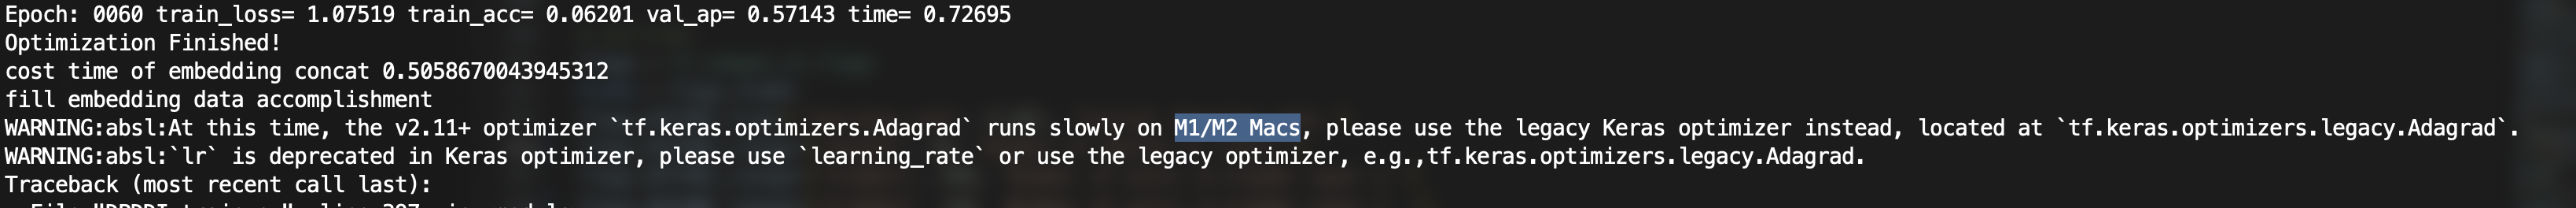
\includegraphics[width=0.9\linewidth]{fig/warning.png}
    \caption{Advertencia de ejecución lenta en chips de arquitectura ARM}
    \label{fig:warninr}
\end{figure}


\chapter{Apéndice: Documentación del código}

Debido a que el código actual no se encuentra adaptado para trabajar con versiones actuales de Python. se realizaron ajustes al mismo que se documentan a continuación:

\begin{figure}
    \centering
    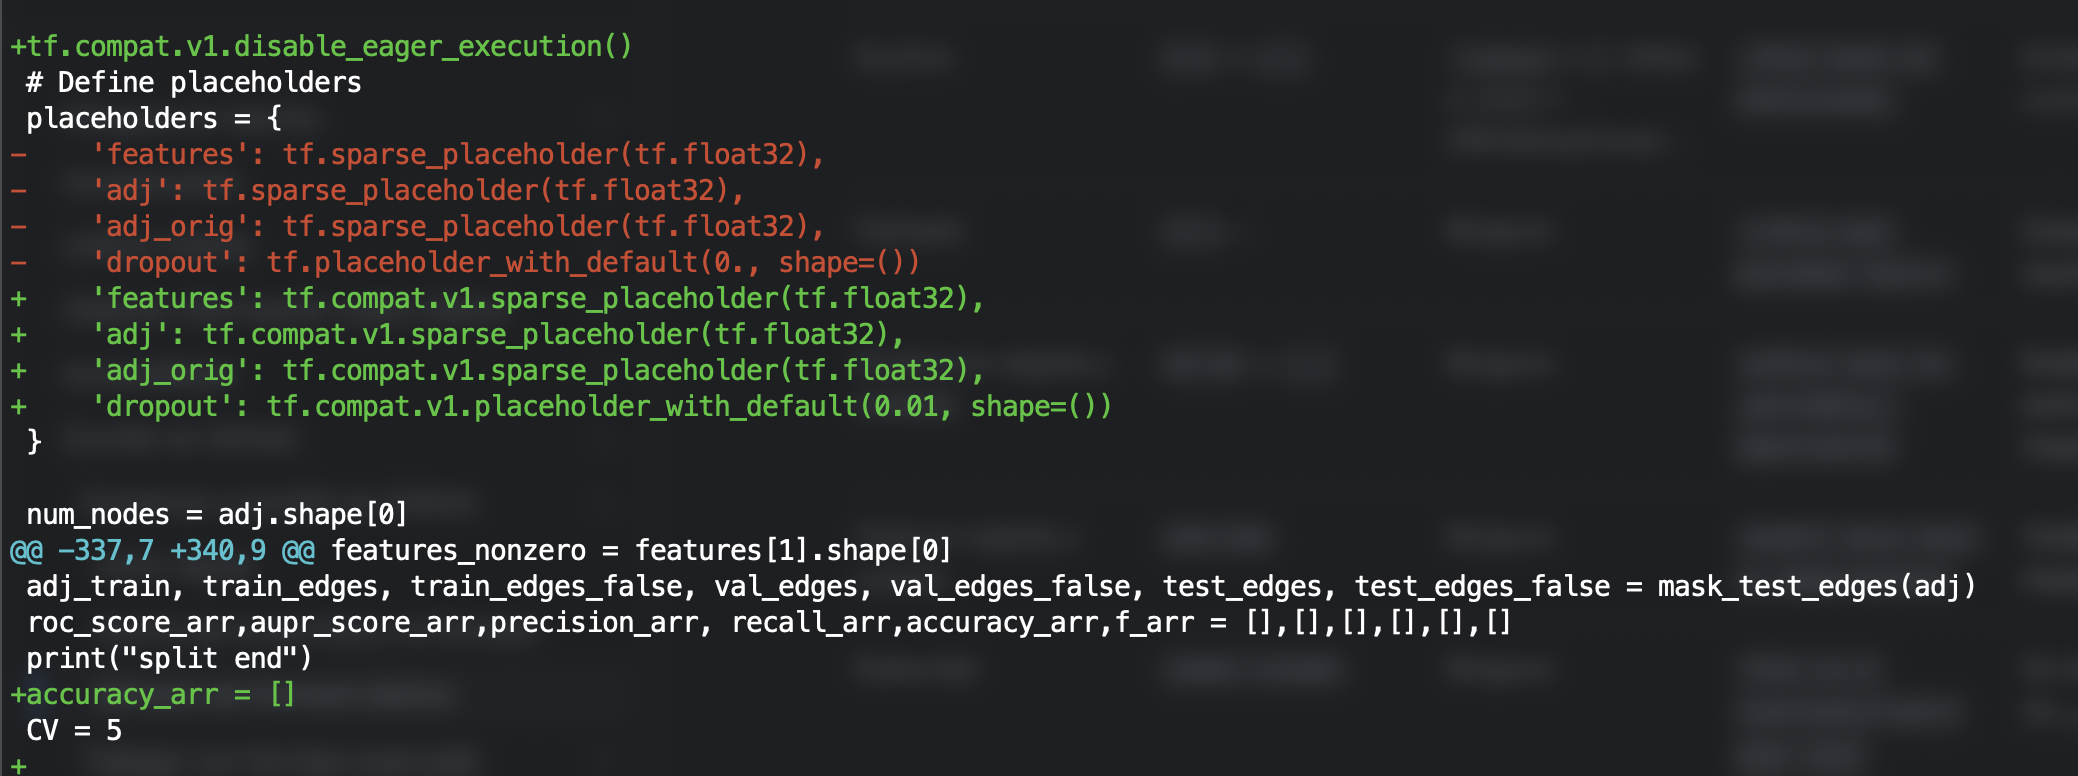
\includegraphics[width=1\linewidth]{fig/code_1.png}
    \caption{Modificación a la compatibilidad del sparse placeholder}
    \label{fig:enter-label}
\end{figure}

\begin{figure}
    \centering
    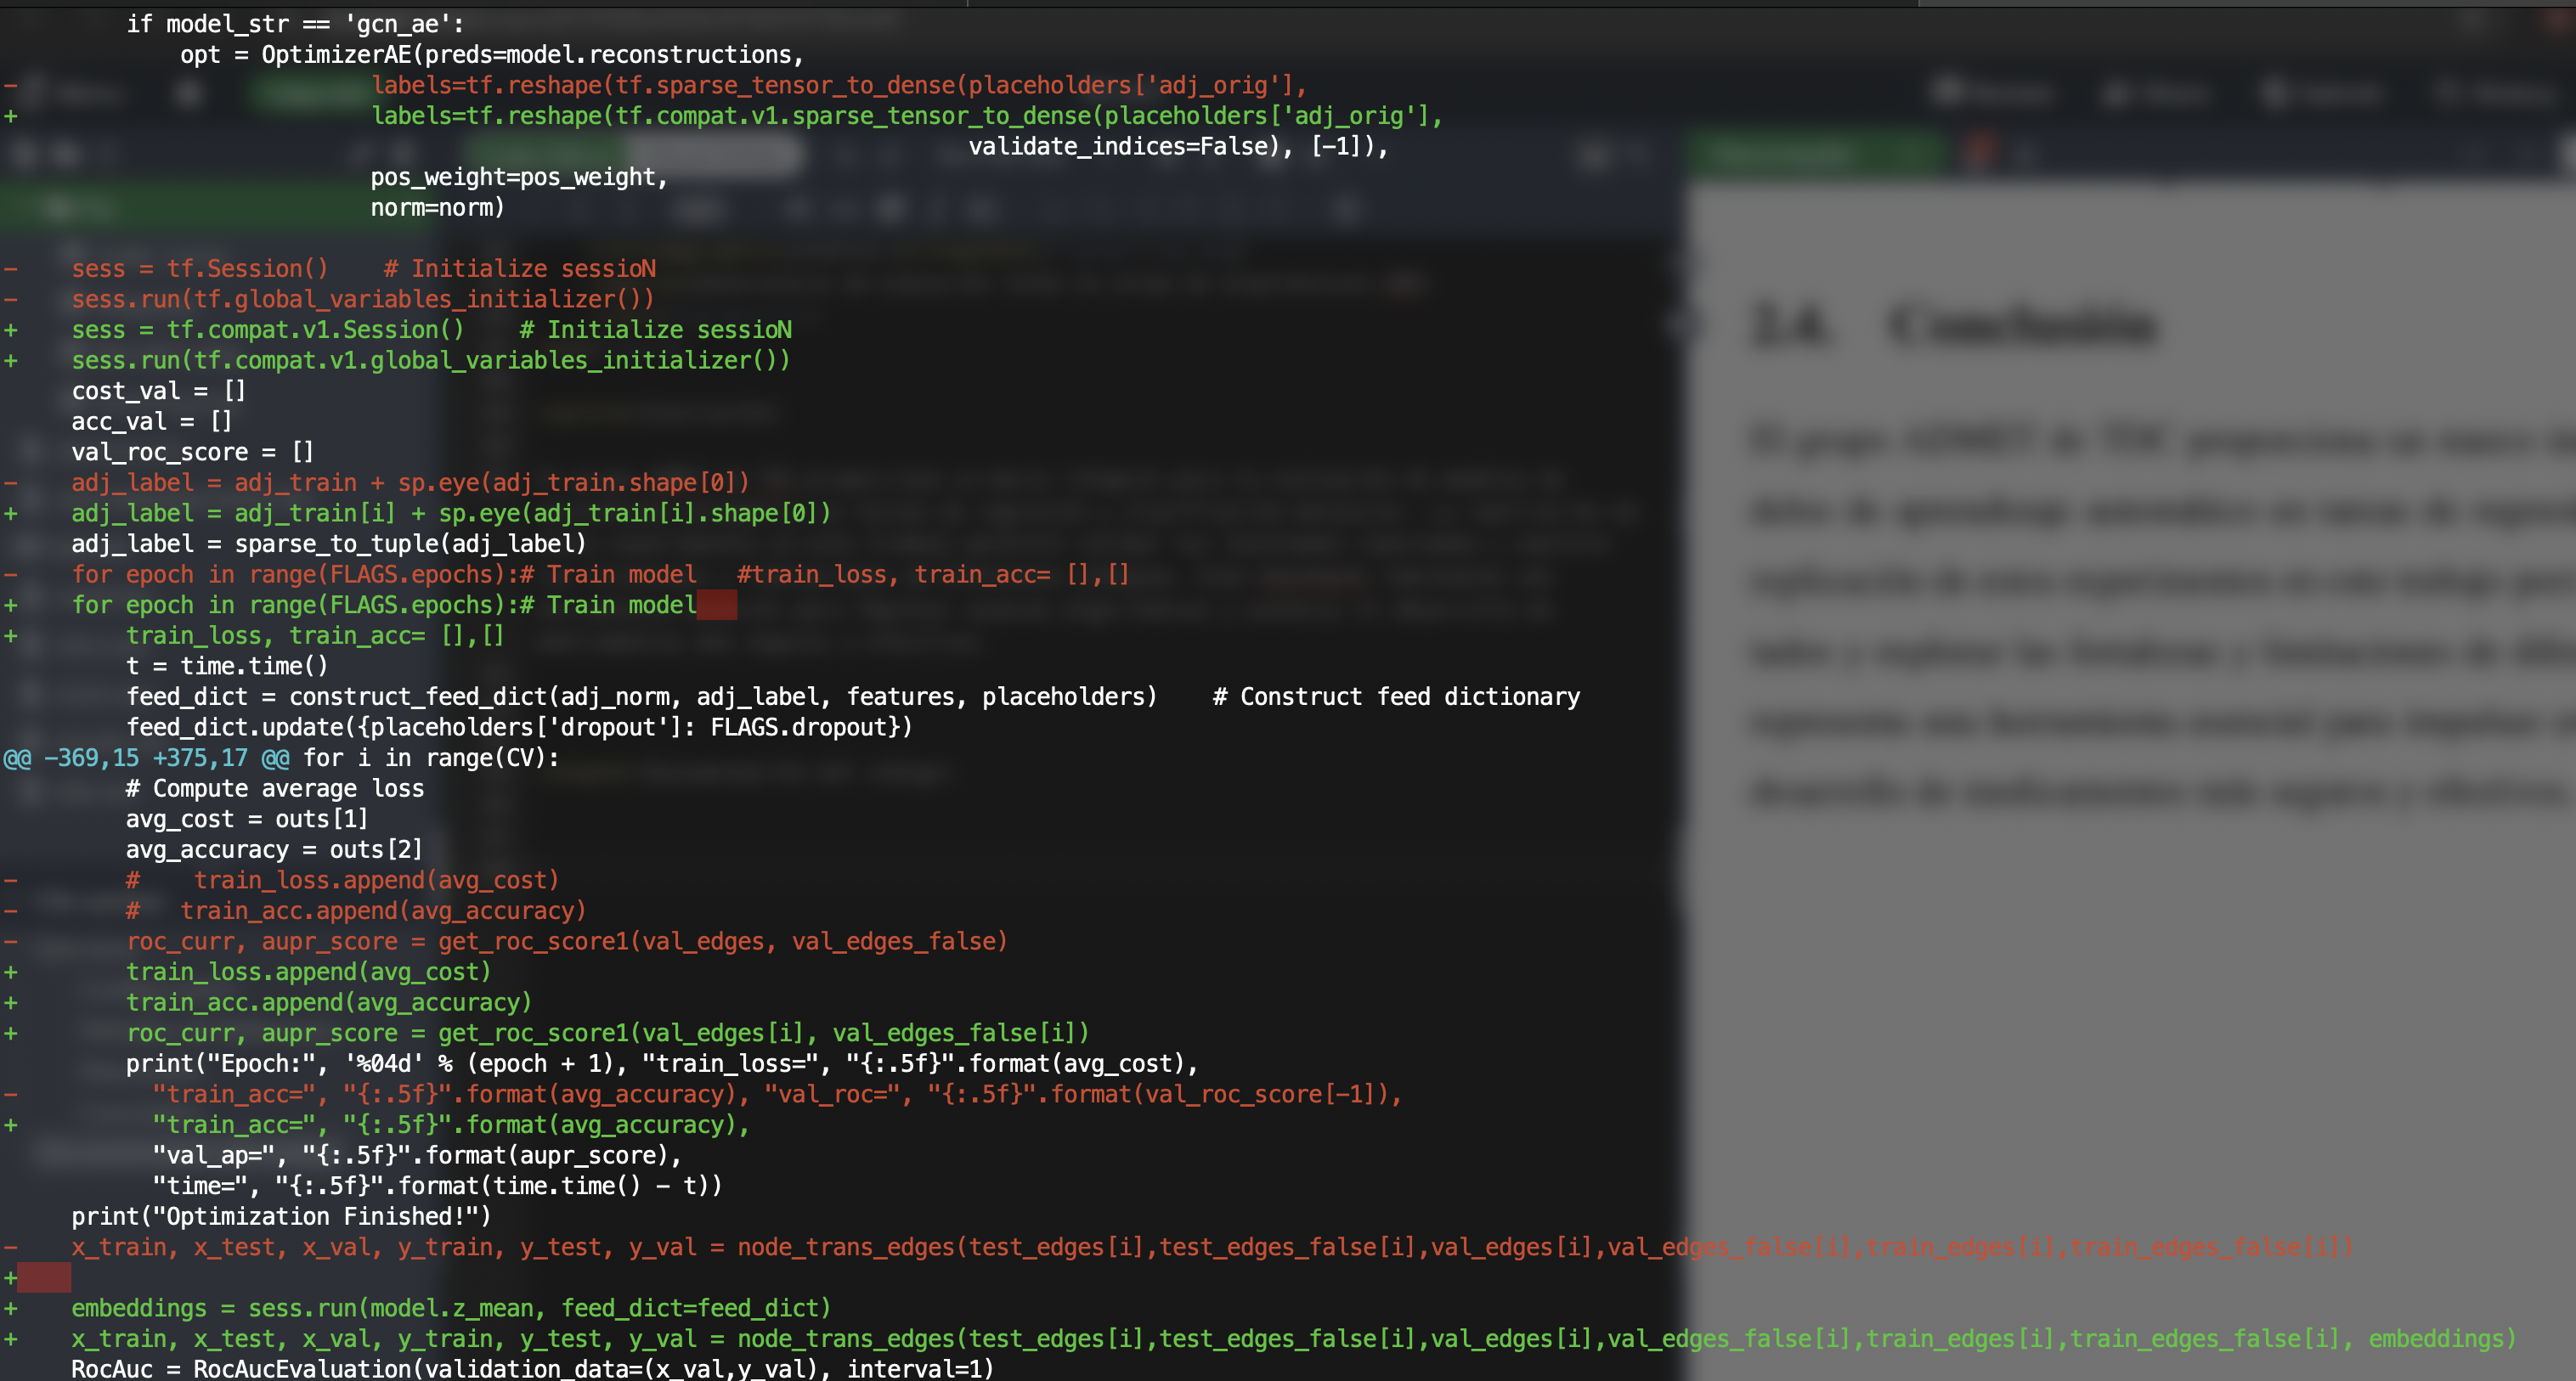
\includegraphics[width=1\linewidth]{fig/code2.png}
    \caption{Modificación a funciones de perdida y formateo de parámetros de accuracy}
    \label{fig:enter-label}
\end{figure}



\begin{figure}
    \centering
    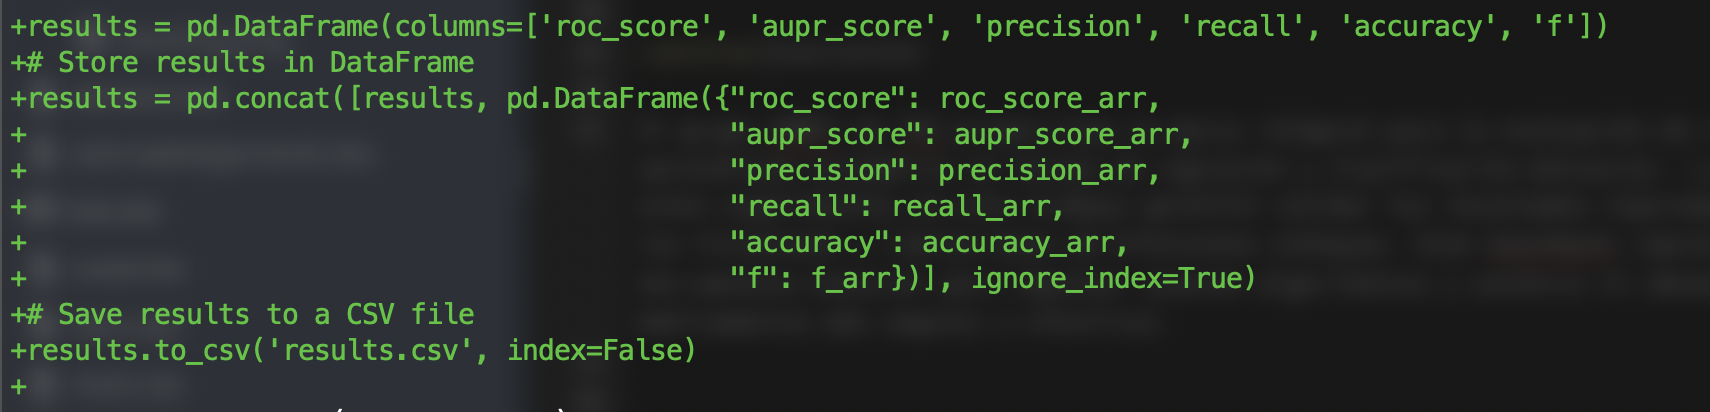
\includegraphics[width=1\linewidth]{fig/code3.png}
    \caption{Nuevo método implementado para almacenar resultados}
    \label{fig:enter-label}
\end{figure}


\begin{figure}
    \centering
    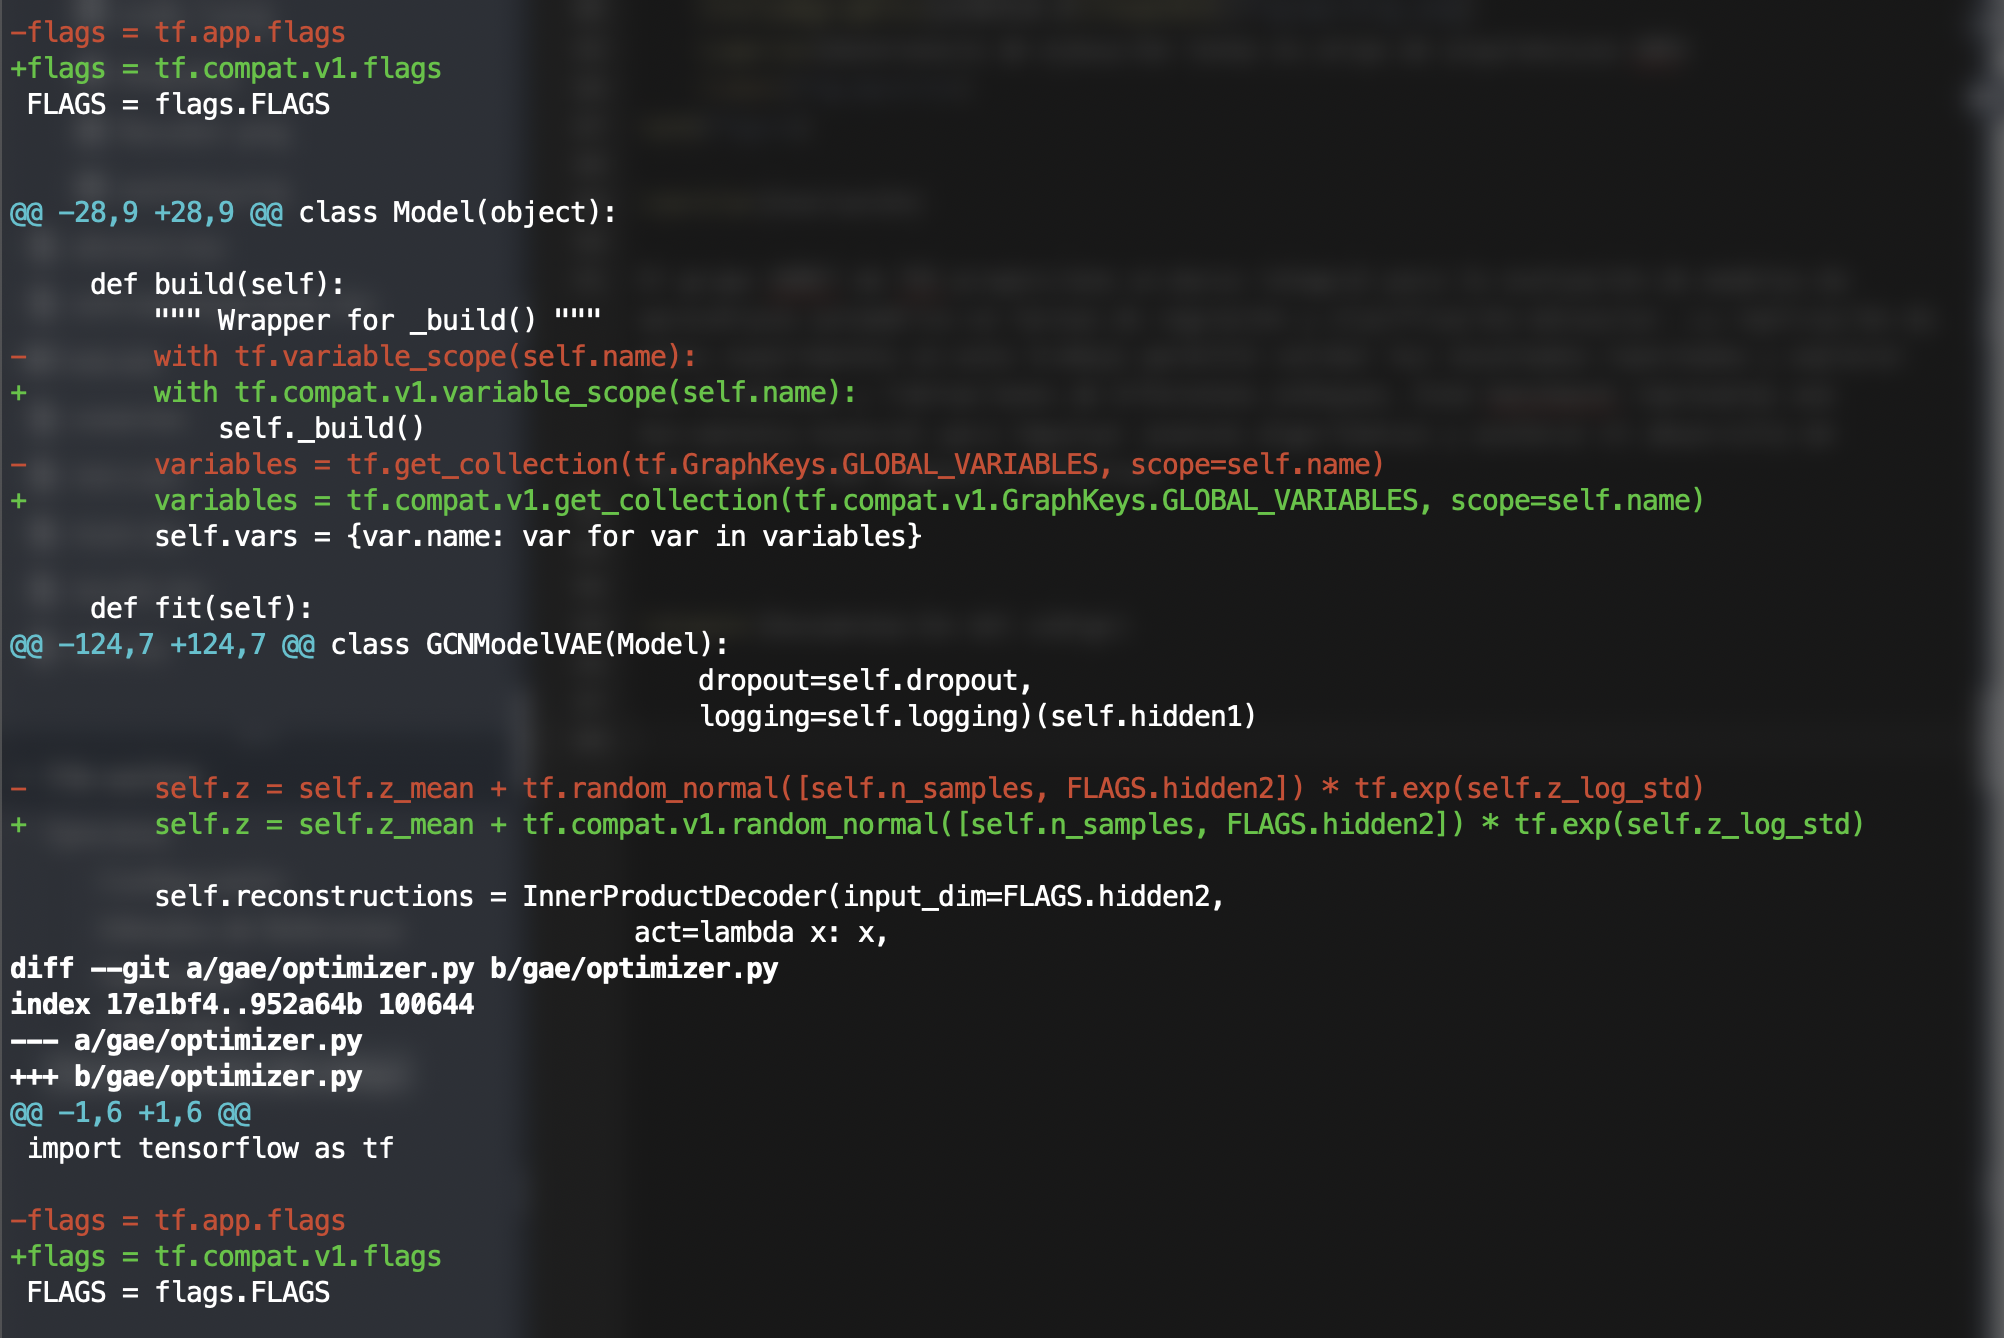
\includegraphics[width=1\linewidth]{fig/code4.png}
    \caption{Modificación a la forma de acceder a las variables flags en las rutinas}
    \label{fig:enter-label}
\end{figure}


\begin{figure}
    \centering
    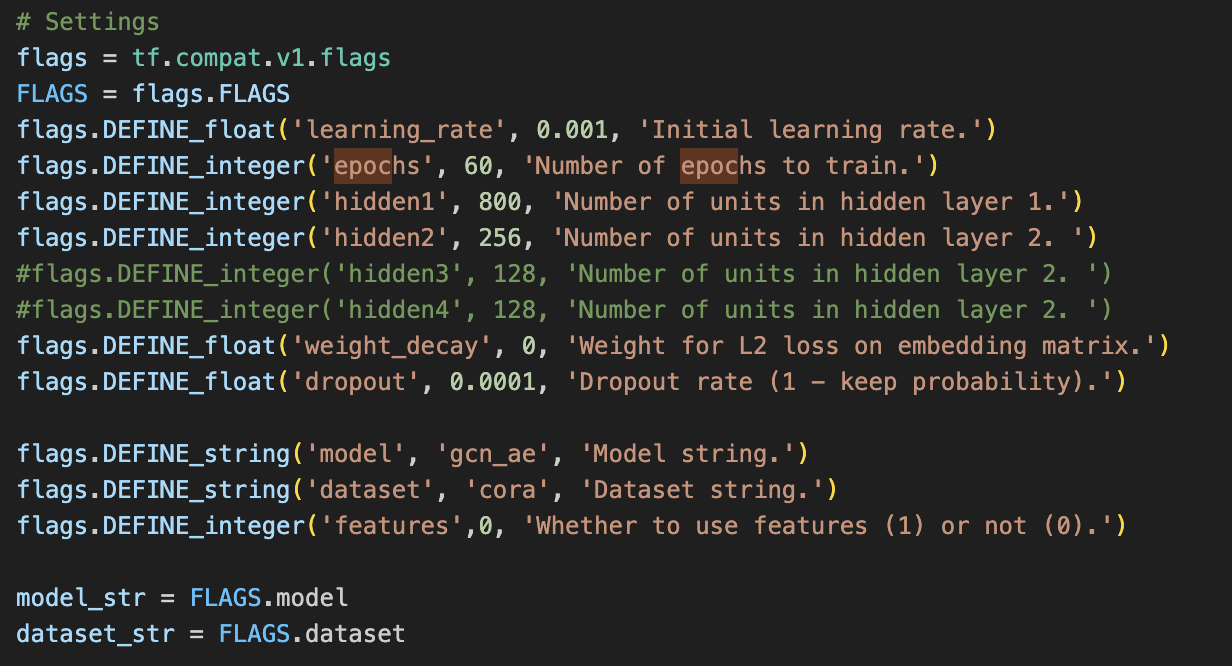
\includegraphics[width=1\linewidth]{fig/epoch.png}
    \caption{Modificación de cantidad de epocas para generar resultados en un tiempo viable
    }
    \label{fig:enter-label}
\end{figure}




\chapter{Benchmarking}

A continuación se presenta la tabla del ejercicio original realizado en el artículo \textbf{Benchmarking Molecular Machine Learning in Therapeutics Data Common}:
\begin{table}[ht]
\centering
\caption{Resultados en el grupo de benchmarks ADMET de TDC. Se reporta el promedio y la desviación estándar en cinco ejecuciones. Las flechas (↑, ↓) indican la dirección de mejor rendimiento. Los mejores métodos están en negritas y los segundos mejores están subrayados.}
\label{tab:admet_results}
\resizebox{\textwidth}{!}{%
\begin{tabular}{lcccccccc}
\toprule
\textbf{Dataset} & \textbf{Metric} & \textbf{Morgan} & \textbf{RDKit2D} & \textbf{CNN} & \textbf{NeuralFP} & \textbf{GCN} & \textbf{AttentiveFP} & \textbf{ContextPred} \\
\midrule
TDC.Caco2 (↓) & MAE & 0.908 ± 0.060 & 0.393 ± 0.024 & 0.446 ± 0.036 & 0.530 ± 0.102 & 0.599 ± 0.104 & 0.401 ± 0.032 & 0.502 ± 0.036 \\
TDC.HIA (↑) & AUROC & 0.807 ± 0.072 & 0.972 ± 0.008 & 0.869 ± 0.026 & 0.943 ± 0.014 & 0.936 ± 0.024 & 0.974 ± 0.007 & 0.975 ± 0.004 \\
TDC.Pgp (↑) & AUROC & 0.880 ± 0.006 & 0.918 ± 0.007 & 0.908 ± 0.012 & 0.902 ± 0.020 & 0.895 ± 0.021 & 0.892 ± 0.012 & 0.923 ± 0.005 \\
TDC.Bioav (↑) & AUROC & 0.581 ± 0.086 & 0.672 ± 0.021 & 0.613 ± 0.013 & 0.632 ± 0.036 & 0.566 ± 0.115 & 0.632 ± 0.039 & 0.671 ± 0.026 \\
TDC.Lipo (↓) & MAE & 0.701 ± 0.009 & 0.574 ± 0.017 & 0.743 ± 0.020 & 0.563 ± 0.023 & 0.541 ± 0.011 & 0.572 ± 0.007 & \textbf{0.535 ± 0.012} \\
TDC.AqSol (↓) & MAE & 1.203 ± 0.019 & 0.827 ± 0.047 & 1.023 ± 0.023 & 0.947 ± 0.016 & 0.907 ± 0.020 & 0.776 ± 0.008 & 1.040 ± 0.045 \\
TDC.BBB (↑) & AUROC & 0.823 ± 0.015 & 0.889 ± 0.016 & 0.781 ± 0.030 & 0.836 ± 0.009 & 0.842 ± 0.016 & 0.855 ± 0.011 & \textbf{0.897 ± 0.004} \\
TDC.PPBR (↓) & MAE & 12.848 ± 0.362 & 9.994 ± 0.319 & 11.106 ± 0.358 & 9.292 ± 0.384 & 10.194 ± 0.373 & 9.373 ± 0.335 & \underline{9.445 ± 0.224} \\
TDC.VD (↑) & Spearman & 0.493 ± 0.011 & 0.561 ± 0.025 & 0.226 ± 0.114 & 0.258 ± 0.162 & 0.457 ± 0.050 & 0.241 ± 0.145 & \underline{0.485 ± 0.092} \\
TDC.CYP2D6-I (↑) & AUPRC & 0.587 ± 0.011 & 0.616 ± 0.007 & 0.544 ± 0.053 & 0.627 ± 0.009 & 0.616 ± 0.020 & 0.646 ± 0.014 & \textbf{0.739 ± 0.005} \\
\bottomrule
\end{tabular}%
}
\end{table}
A continuación se presentan los resultados para la replicación de los resultados.


\begin{table}[ht]
\centering
\label{tab:admet_metrics}
\begin{tabular}{|l|c|c|}
\hline
\textbf{Dataset} & \textbf{Media} & \textbf{Desviación Estándar} \\ \hline
caco2\_wang & 0.932 & 0.061 \\ \hline
hia\_hou & 0.806 & 0.068 \\ \hline
pgp\_broccatelli & 0.878 & 0.010 \\ \hline
bioavailability\_ma & 0.553 & 0.094 \\ \hline
lipophilicity\_astrazeneca & 0.702 & 0.014 \\ \hline
solubility\_aqsoldb & 1.196 & 0.010 \\ \hline
bbb\_martins & 0.816 & 0.012 \\ \hline
ppbr\_az & 12.841 & 0.463 \\ \hline
vdss\_lombardo & 0.476 & 0.032 \\ \hline
cyp2d6\_veith & 0.582 & 0.013 \\ \hline
cyp3a4\_veith & 0.833 & 0.005 \\ \hline
cyp2c9\_veith & 0.719 & 0.008 \\ \hline
cyp2d6\_substrate\_carbonmangels & 0.669 & 0.036 \\ \hline
cyp3a4\_substrate\_carbonmangels & 0.638 & 0.011 \\ \hline
cyp2c9\_substrate\_carbonmangels & 0.382 & 0.011 \\ \hline
half\_life\_obach & 0.374 & 0.058 \\ \hline
clearance\_microsome\_az & 0.505 & 0.015 \\ \hline
clearance\_hepatocyte\_az & 0.270 & 0.069 \\ \hline
herg & 0.715 & 0.032 \\ \hline
ames & 0.801 & 0.009 \\ \hline
dili & 0.828 & 0.015 \\ \hline
ld50\_zhu & 0.642 & 0.020 \\ \hline
\end{tabular}
\caption{Resultados de los benchmarks ADMET con la red MORGAN con sus medias y desviaciones estándar.}
\end{table}

A continuación se muestran los resultados obtenidos directamente de la consola de ejecución:

\begin{figure}
    \centering
    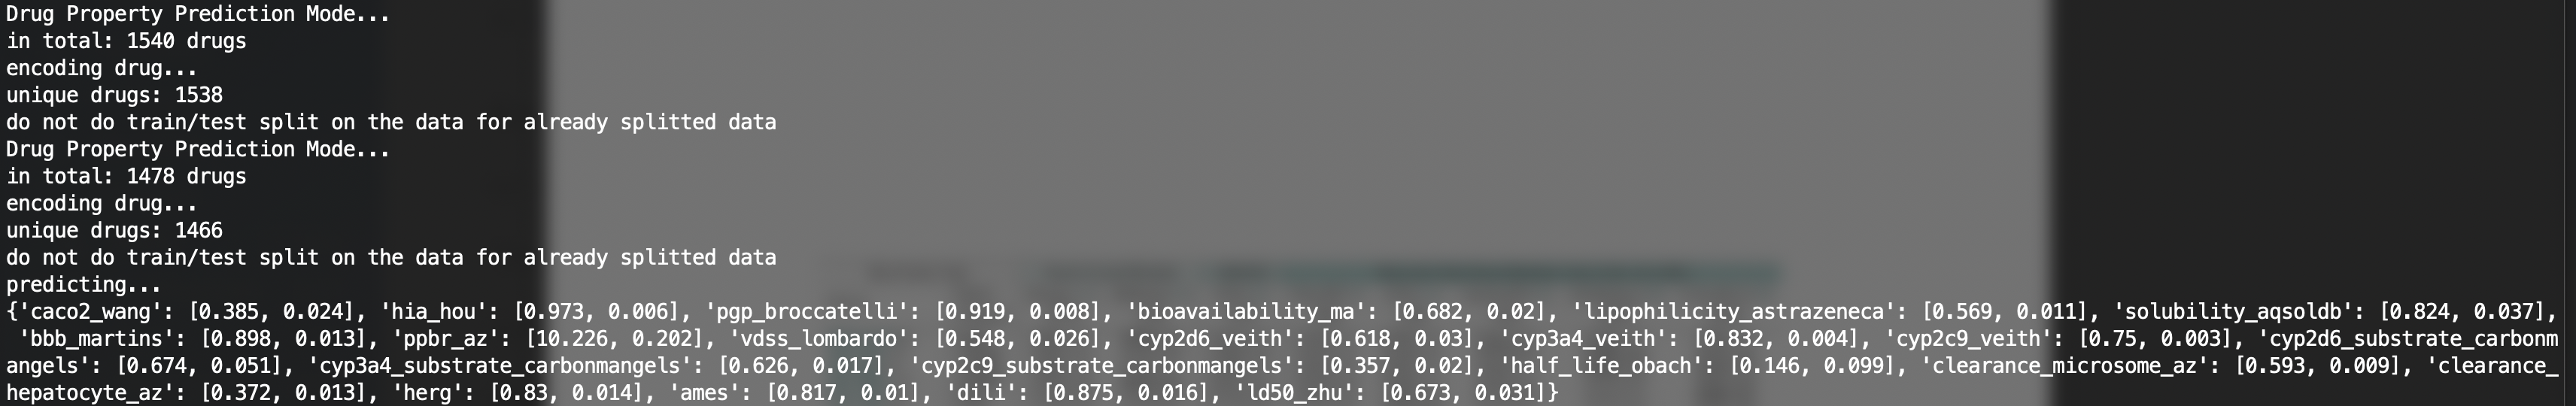
\includegraphics[width=1\linewidth]{fig/Results1.png}
    \caption{Ejecución de benchmark con red Morgan}
    \label{fig:enter-label}
\end{figure}